\newpage
\section{Developing the game}
While developing the gamepad driver, we also began prototyping the game.
Since we had an existing implementation of the game \cite{2048} to reference,
the game mechanics were fairly straightforward to implement.

As the entire source code of the game is quite large, this section will only discuss the more (in our opinion) interesting parts of it.
The entire source code is attached to the report.

\subsection{Game board data structure\label{data_structure}}
The game is based around a simple 16-slot array representing a four by four grid of numbers.
Button presses causes the numbers to move around and merge,
and the updated array is translated to graphics that are shown on the gameboard screen.

Since the board was only to contain values of the form $v = 2^n$, it made sense to store $n$ instead of $v$. Only the case of $n = 0$ is different, as these are not to be displayed as tiles with the value $1$, but rather as empty tiles.

\begin{table}[h!]
    \centering
    \begin{tabular}{|l|l|l|l|l|l|l|l|l|l|l|l|l|l|l|l|}
        \hline
        0 & 0 & 0 & 1 & 0 & 1 & 2 & 1 & 0 & 0 & 2 & 4 & 2 & 5 & 8 & 5 \\ \hline
    \end{tabular}
    \caption{An example of how the array \texttt{uint8\_t b[16]} could look.}
    \label{array_b}
\end{table}

\begin{figure}[h!]
    \centering
    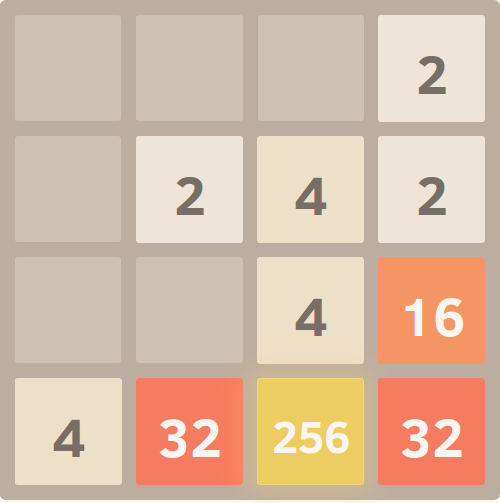
\includegraphics[width=5cm]{img/2048.png}
    \caption{How the screen representation of the \texttt{b} array (table \ref{array_b}) would look.}
\end{figure}

\newpage
\subsection{Gamepad input}
\label{gamepad-input}
Upon starting the game program, the gamepad driver listening is initialized by the function \texttt{init\_gamepad}.

\noindent{
\begin{minipage}{\linewidth}
\begin{lstlisting}[language=C, label=init_gamepad, caption=Initializing the gamepad driver listening]
int init_gamepad()
{
    device = fopen("/dev/gamepad", "rb");
    if (!device) {
        printf("Unable to open driver device, maybe you didn't load the module?\n");
        return EXIT_FAILURE;
    }
    if (signal(SIGIO, &sigio_handler) == SIG_ERR) {
        printf("An error occurred while register a signal handler.\n");
        return EXIT_FAILURE;
    }
    if (fcntl(fileno(device), F_SETOWN, getpid()) == -1) {
        printf("Error setting pid as owner.\n");
        return EXIT_FAILURE;
    }
    long oflags = fcntl(fileno(device), F_GETFL);
    if (fcntl(fileno(device), F_SETFL, oflags | FASYNC) == -1) {
        printf("Error setting FASYNC flag.\n");
        return EXIT_FAILURE;
    }
    return EXIT_SUCCESS;
}
\end{lstlisting}
\end{minipage}
}


This sets up the program so that when the driver registers an interrupt, the function \texttt{sigio\_handler()} is called.

\noindent{
\begin{minipage}{\linewidth}
\begin{lstlisting}[language=C, label=sigio_handler, caption=Input handler function]
void sigio_handler(int signo)
{
    int input = map_input(fgetc(device));
    switch (input) {
        case 1:
            left();
            break;
        case 2:
            up();
            break;
        case 3:
            right();
            break;
        case 4:
            down();
            break;
        case 6:
            if (last_input == 6) {
                new_game();
            }
            break;
        case 8:
            if (last_input == 8) {
                running = false;
            }
            break;
    }
    last_input = input;
}

\end{lstlisting}
\end{minipage}
}

The gamepad driver is accessed in the handler with \texttt{fgetc(device)}, which returns a bit string that represents the state of each of the eight buttons.
For this game, we were not interested in any button press combinations, so we used the function we defined in exercise 2 to map the input to a number representing a single button pressed.

\noindent{
\begin{minipage}{\linewidth}
\begin{lstlisting}[language=C, label=map_input, caption=Input decoding function]
int map_input(int input)
{
    input = ~input;
    for ( int i = 0; i < 8; i++) {
        int match = input & (1 << i);
        if ( (1 << i) == match ) {
            return (i+1);
        }
    }
    return 0;
}
\end{lstlisting}
\end{minipage}
}


The main function of the game has a loop that suspends at the end of each iteration.
When the driver registers an interrupt it is handled by the handler function, then the main loop updates the screen contents and suspends again.

\newpage
\subsection{Using the development board LED display}
As advised in the compendium, we used memory mapping to manipulate the image to be displayed.

\noindent{
\begin{minipage}{\linewidth}
\begin{lstlisting}[language=C, label=init_framebuffer, caption=Framebuffer initializing function]
int init_framebuffer()
{
    fbfd = open("/dev/fb0", O_RDWR);
    if (fbfd == -1) {
        printf("Error: unable to open framebuffer device.\n");
        return EXIT_FAILURE;
    }

    // Get screen size info
    if (ioctl(fbfd, FBIOGET_VSCREENINFO, &vinfo) == -1) {
        printf("Error: unable to get screen info.\n");
        return EXIT_FAILURE;
    }

    screensize_pixels = vinfo.xres * vinfo.yres;
    screensize_bytes = screensize_pixels * vinfo.bits_per_pixel / 8;

    fbp = (uint16_t*)mmap(NULL, screensize_bytes, PROT_READ | PROT_WRITE, MAP_SHARED, fbfd, 0);
    if ((int)fbp == MAP_FAILED) {
        printf("Error: failed to memorymap framebuffer.\n");
        return EXIT_FAILURE;
    }

    return EXIT_SUCCESS;
}
\end{lstlisting}
\end{minipage}
}


This maps a region of memory, identified by the pointer \texttt{fbp}, to \texttt{/dev/fb0}, the interface for manipulating the development board LED display.
Each 16-bit integer in this region represents the RGB565 color of a single pixel.
With this we were now able to draw shapes by iterating over the memory region and writing different values.
After changing pixels, the function \texttt{ioctl(fbfd, FB\_DRAW, \&screen)} is called to tell the screen to refresh the pixels in the \texttt{screen} area.

One thing we noticed and were confused by for quite some time was a black square region of ~5-10 pixels that would not go away.
It was eventually revealed to us that this was a cursor that uCLinux placed on the screen.
We were also told that this could be removed by running the command \texttt{echo 0 > /sys/class/graphics/fbcon/cursor\_blink} on the board.


\newpage
\subsection{Using fonts}

With a game relying as strongly on text for both user feedback and main game elements as ours, we quickly realised we would need a well structured way of defining fonts. We also wanted to be able to use different font sizes. 
While we could have gotten away with defining some sort of array representation of each letter of a font in a header file, we also wanted to be able to edit fonts in any modern image editor. We started investigating various simple image formats to this end.

The first problem we bumped into, was how to get the image files we needed onto the root file system and transferred to the board. The compendium offered little to no guidance on the subject, but having familiarized ourselves with the PTXdist build system, we knew we would have to amend the \texttt{rules/game.make} file. We consulted the PTXdist application note; "How to become a PTXdist Guru" \cite{ptxdistguru}, and found what we were looking for. Listing \ref{image-build} shows how we accomplished this.

\noindent{
\begin{minipage}{\linewidth}
\begin{lstlisting}[label=image-build, caption=Including images]
RESOURCES_DIR   := local_src/$(GAME)-$(GAME_VERSION)/res
@$(call install_copy, game, 0, 0, 0755, $(RESOURCES_DIR)/font/font_large.pbm, /lib/$(GAME)/res/font/font_large.pbm)
\end{lstlisting}
\end{minipage}
}



We first attempted to use the BMP format, and wrote quite a bit of code parsing this format, but after several hours of banging our heads against the wall, we decided to look for something simpler. 
The BMP format contains a little too much information about things we would never have any use for, like color depth, color planes, print resolution, etc.

We decided to use the Portable bitmap format (.pbm).
This is a much simpler format than the normal bitmap format (.bmp),
yet offers everything we need.
Files in the .pbm format have some header data first, then a sequence of 1s and 0s that represent a simple monochrome image.
For instance, the data for a very simple .pbm image is shown in listing \ref{pbm-image}

\noindent{
\begin{minipage}{\linewidth}
\begin{lstlisting}[label=pbm-image, caption=PBM image]
P1
# This is an example bitmap of the letter "J"
6 10
0 0 0 0 1 0
0 0 0 0 1 0
0 0 0 0 1 0
0 0 0 0 1 0
0 0 0 0 1 0
0 0 0 0 1 0
1 0 0 0 1 0
0 1 1 1 0 0
0 0 0 0 0 0
0 0 0 0 0 0
\end{lstlisting}
\end{minipage}
}

We procured some pixel fonts in .bmp format online, then converted them to .pbm and included with the flash.

First we needed to read the pbm file, parse the data and store it to memory.
We created a simple struct to hold the data.

\noindent{
\begin{minipage}{\linewidth}
\begin{lstlisting}[language=C, label=pbm_image_t, caption=Portable bitmap format data struct]
typedef struct {
    unsigned int x;
    unsigned int y;
    bool* data;
} pbm_image_t;

\end{lstlisting}
\end{minipage}
}


Refer to the attached source code for the \texttt{path\_to\_pbm} function in the file \texttt{font.c}.
It is a bit too long to include in this report, but what it does is simply read a .pbm file and parse the sequence of 1s and 0s into the boolean array \texttt{pbm\_image\_t->data}.

Next up was to separate the data we now had in memory into individual boolean arrays representing individual character masks.
Again we created a simple struct that could hold the boolean data for the character mask.

\noindent{
\begin{minipage}{\linewidth}
\begin{lstlisting}[language=C, label=char_t, caption=Character mask struct]
typedef struct {
    char name;
    bool* data;
} char_t;
\end{lstlisting}
\end{minipage}
}


In addition we created another struct to hold the collection of different character masks (a font).

\noindent{
\begin{minipage}{\linewidth}
\begin{lstlisting}[language=C, label=font_t, caption=Font struct]
typedef struct {
    unsigned int char_w;
    unsigned int char_h;
    char_t* chars;
} font_t;
\end{lstlisting}
\end{minipage}
}


The function \texttt{pbm\_to\_font} (also in \texttt{font.c}) iterates over the \texttt{pbm\_image\_t->data} array and creates \texttt{char\_t} objects for the characters \texttt{' '} through \texttt{'z'} (ASCII ordering) and stores these in a single font.
After this the memory holding the \texttt{pbm\_image\_t} data is freed.

% glyph stuff in next subsection


\newpage
\subsection{Using the development board LED display}
As advised in the compendium, we used memory mapping to manipulate the image to be displayed.

\noindent{
\begin{minipage}{\linewidth}
\begin{lstlisting}[language=C, label=init_framebuffer, caption=Framebuffer initializing function]
int init_framebuffer()
{
    fbfd = open("/dev/fb0", O_RDWR);
    if (fbfd == -1) {
        printf("Error: unable to open framebuffer device.\n");
        return EXIT_FAILURE;
    }

    // Get screen size info
    if (ioctl(fbfd, FBIOGET_VSCREENINFO, &vinfo) == -1) {
        printf("Error: unable to get screen info.\n");
        return EXIT_FAILURE;
    }

    screensize_pixels = vinfo.xres * vinfo.yres;
    screensize_bytes = screensize_pixels * vinfo.bits_per_pixel / 8;

    fbp = (uint16_t*)mmap(NULL, screensize_bytes, PROT_READ | PROT_WRITE, MAP_SHARED, fbfd, 0);
    if ((int)fbp == MAP_FAILED) {
        printf("Error: failed to memorymap framebuffer.\n");
        return EXIT_FAILURE;
    }

    return EXIT_SUCCESS;
}
\end{lstlisting}
\end{minipage}
}


This maps a region of memory, identified by the pointer \texttt{fbp}, to \texttt{/dev/fb0}, also known as the development board LED display.
Each 16-bit integer in this region represents the RGB565 color of a single pixel on the screen.
With this we were now able to draw shapes by iterating over the memory region and writing different values.
After changing pixels, the function \texttt{ioctl(fbfd, FB\_DRAW, \&screen)} is called to tell the screen to refresh the pixels in the \texttt{screen} area.

\subsection{Putting everything together}
Now, with easy control of every single individual pixel and multiple fonts loaded into memory, we were ready to put everything together to make our game more or less equivalent to the web game.

The first step towards putting text on the screen was to put multiple character masks together into a single mask representing a string.
This mask of multiple characters we called a glyph, and we created a function that would create a glyph from a string of arbitrary length and a font.

\noindent{
\begin{minipage}{\linewidth}
\begin{lstlisting}[language=C, label=create_glyph, caption=Glyph creation function]
bool* create_glyph(char* str, int len, font_t* font)
{
    bool* glyph = (bool*)malloc(len*(font->char_h)*(font->char_w)*sizeof(bool));
    for (int i = 0; i < len; i++) {
        bool* chardata = font->chars[str[i]-' '].data;
        for (int y = 0; y < (font->char_h); y++) {
            for (int x = 0; x < (font->char_w); x++) {
                glyph[(len * (font->char_w) * y) + i*(font->char_w) + x] = chardata[(font->char_w)*y + x];
            }
        }
    }

    return glyph;
}
\end{lstlisting}
\end{minipage}
}


With this we could now draw the game board from the values in the array \texttt{b} (section \ref{data_structure}).
From the position in the array we calculated the 60x60 pixel area of the framebuffer corresponding, and in this we drew a square colored according to the value in the array.
In the centre of the square we drew a glyph created from the string representation of the value in the array.

\noindent{
\begin{minipage}{\linewidth}
\begin{lstlisting}[language=C, label=draw_tile, caption=Tile drawing function]
void draw_tile(int pos, int val)
{
    int number = pow(2, val);

    int screen_offset_x = (60 * pos) % 240;
    int screen_offset_y = 60 * (pos / 4) - 1;

    int len = 0;
    if (val > 0) {
        int temp = number;
        while(temp) {
            temp = temp / 10;
            len++;
        }
    } else {
        len = 1;
    }

    char str[len];
    sprintf(str, "%d", number);

    int padding_y = (60 - (font->char_h)) / 2;
    int padding_x = (60 - len*(font->char_w)) / 2;

    bool* glyph = create_glyph(str, len, font);

    for (int y = MARGIN; y < 60 - MARGIN; y++) {
        for (int x = MARGIN; x < 60 - MARGIN; x++) {
            int screen_index = vinfo.xres*(y + screen_offset_y) + x + screen_offset_x;

            bool g = glyph[(y-padding_y)*len*(font->char_w) + (x-padding_x)];
            bool b = padding_y < y && y < 60 - padding_y && padding_x < x && x < 60 - padding_x;
            if (val != 0 && g && b) {
                fbp[screen_index] = Black; // glyph color
            } else {
                fbp[screen_index] = colors[val]; // tile bg color
            }
        }
    }
    free(glyph);
}
\end{lstlisting}
\end{minipage}
}

